\documentclass{article}
\usepackage{amsmath}
\usepackage{amsthm}
\usepackage{amsfonts}
\usepackage{physics}
\usepackage{siunitx}
\usepackage{graphicx}
\usepackage{hyperref}
\usepackage{natbib}
\usepackage[english]{babel}
\usepackage[autostyle, english = american]{csquotes}
\usepackage[margin=1in]{geometry}
\MakeOuterQuote{"}

\newtheorem{definition}{Definition}[section]
\newtheorem{theorem}{Theorem}[section]
\newtheorem{proposition}{Proposition}[section]
\newtheorem{lemma}{Lemma}[section]
\newtheorem{corollary}{Corollary}[section]
\newtheorem{example}{Example}[section]
\newtheorem{algorithm}{Algorithm}[section]
\newtheorem{remark}{Remark}[section]

\newcommand{\R}{\mathbb{R}}
\newcommand{\C}{\mathbb{C}}
\newcommand{\Z}{\mathbb{Z}}
\newcommand{\x}{\vb{x}}
\newcommand{\y}{\vb{y}}
\newcommand{\w}{\vb{w}}
\newcommand{\0}{\vb{0}}
\newcommand{\h}{\vb{h}}

\bibliographystyle{apalike}

\graphicspath{{../}}

\title{A Crash Course in Numerical Methods for Initial Value Problems \\ \small{How to make a computer do horrible math for you}}
\author{Ben Goldman}

\begin{document}
\maketitle

\abstract{
  Ordinary differential equations are fundamental to nearly all applications of mathematics, especially physics, in which one must work backwards from a known function of derivatives of an unknown function. However, many ordinary differential equations that appear in applications lack a closed-form solution. Scientists employ numerical methods to approximately solve these problems, enabling the computational simulation of nearly any physical system. Here I present the most frequently-used numerical tools for ordinary differential equations and analyze their properties. This paper assumes a background in differential calculus, through Taylor's Theorem. Example implementation is located \href{https://github.com/ben-goldman/ode}{here}.
}

\section{Motivation: why we want numerical methods for ODE's}

\subsection{Formulating the problem}

Most problems in physics are presented in an ordinary differential equation (ODE), in which a function relating the derivatives of an unknown function is known. Formally stated, an ODE looks like this:

\begin{definition}
  Given a function $f: U \subset \R^{n+1} \to \R$, an  \textbf{ordinary differential equation (ODE) of degree $n$} is an equation of the form
  \[0 = f\mqty(t, y, y', \cdots, y^{(n)})\]
  where $y$ is some $C^n$ function $y: \R\to\R$.
\end{definition}

\begin{example}
  The equation $y'' + 2y - e^{\tan^{-1}(\sqrt{y'''})} = \sin(1/y + \cos(t)) - \ln(y^t)$ is a third-order ODE that corresponds to the equation
  \[f(t, y, y', y'', y''') = y'' + 2y - e^{tan^{-1}(\sqrt(y'''))} - \sin(\frac{1}{y} + \cos(t)) + \ln(y^t) = 0\]
\end{example}

Given such a problem, we can define the solution as:
\begin{definition}
  A $C^n$ function $u: (a, b)\to\R$ is a \textbf{solution} to the ODE $f(t, y', \cdots, y^{(n)}) = 0$ if:
  \[f\qty(t, u(t), u'(t), \cdots, u^{(n)}(t)) = 0\]
\end{definition}

\begin{example}
  The function $u(t) = e^{-ct}$ is a solution to the first-order ODE $y' + cy = 0$ because $u'(t) - u(t) = \dv{t}(e^{-ct}) - ce^{-ct} = -ce^{-ct} + ce^{-ct} = 0$.
\end{example}

Such a problem can be generalized to vector valued functions $y: \R \to \R^m$, where
\[y(t) = \mqty(y_1(t)\\\vdots\\y_m(t)).\]

\begin{definition}
  Given a function $f: U \subset \R\times(\R^m)^n \to \R^m$ a \textbf{system of $m$ differential equations of order $n$} is the equation
  \[f(t, y, y', \cdots, y^{(n)}) = \0\]
  where $u: I\subset\R \to \R^m$ is a solution if
  \[f\qty(t, u(t), u'(t), \cdots, u^{(n)}(t)) = \0\]
\end{definition}

\begin{example}
  The system
  \[\mqty(x'\\y'\\z') = \mqty(10(y-x)\\x(28-z) - y\\xy - \frac{8}{3} z) \qquad \mqty(x(0)\\y(0)\\z(0)) = \mqty(0\\0\\28)\]
  is an initial value problem over a simple system of ordinary differential equations that has a fun and disturbing solution.
\end{example}

However, there is no guarantee that an ODE admits a unique solution, or a solution at all. However, in well-behaved cases, by specifying the value of the solution at a single point, we can guarantee a unique solution, (see \autoref{plt}).

\begin{definition}
  An \textbf{Initial Value Problem (IVP)} is a first order ordinary differential equation with $U = [a, b]\times\R^n$ and $f: U\to\R^n$
  \[y'(t) = f(t, y(t))\]
  when for some $t_0 \in [a, b]$ we have
  \[y(t_0) = y_0\]
\end{definition}

Now that we know what an ODE looks like, we'll want to look for ways of solving them. First, I'll present a few examples of problems in which ODE's arise to motivate the use of numerical methods in their solution.

\subsection{Motivating example: pendulums}

Say we have an (ideal) pendulum: a mass suspended by a massless rigid bar subject to a gravitational force. We want to find the evolution of the angle of the mass given an initial angle and velocity. For simplicity's sake, assume the mass to be $\SI{1}{\kilo\gram}$, the string's length to be $\SI{1}{\meter}$ and the strength of gravity to be $\SI{1}{\meter\per\second^2}$. The mass has an angle from the vertical $\theta(t)$, and begins with an initial angle $\theta_0 \in [-\pi, \pi]$. Then we release the mass and it swings back and forth. It can be shown that the mass obeys the following equation of motion:
\[\dv[2]{\theta}{t} = -\sin\theta \qquad \theta(0) = \theta_0, \theta'(0) = 0\]
We can phrase this as the $2^{nd}$ order ODE
\[\theta'' + \sin\theta = 0\]
which can be reduced to the $1^{st}$ order system
\[\mqty(x'(t)\\y'(t)) = \mqty(y(t)\\-\sin x(t))\]
Due to the nonlinear behavior of the $\sin\theta$ term, this equation is incredibly difficult to solve analytically. For situations in which $\theta_0 \approx 0$ we can use the first order taylor expansion $\sin\theta \approx \theta$ to produce an approximate solution to this equation:
\[\theta(t) \approx \theta_0\cos(t)\]
ODE's where analytical solutions are unwieldy, if not imposible, dominate science. In these cases, the best way to determine the behavior of the solution is through numerical calculations. We trade not knowing the exact symbolic form of the solution for at least knowing its value over a range of points. Therefore, the ability to produce numerical results for the solution of an initial value problem has immense utility.

\section{How computers do math}

Obviously you don't want to do all those computations by hand---so we turn to computers. Unfortunately, as we will see, computers are always a little bit wrong. Therefore, a good computer program should be \emph{convergent}: we should be able to keep the error under control. While computers are fast at math, solving an ODE requires a lot of calculations. Therefore, we also want our algorithms to run \emph{quickly}. Finally, computers have limited processing and storage capacity. Therefore, a good algorithm runs \emph{efficiently}. Let's address these requirements.

\subsection{Floating-point numbers and round-off error}

Computers represent all numbers with limited precision. The dominant method for encoding the reals is through floating-point representation. To a high level of abstraction, computers represent numbers the same way as humans do when using scientific notation. They write a number as a number times a base raised to an exponent. However, like humans using paper, these numbers can only fit in a finite set of storage. Therefore, we define the set of numbers representable on a computer as the following:
\begin{definition}
  Given a computer with $p$-bit precision, the set of \textbf{floating-point numbers} is the set of numbers precicely representable on such a computer, given by the set
  \[F_p = \qty{M\times 2^E | M \in \Z, E \in \Z, \substack{|M| < 2^p \\ |E| < 2^p}}\]
\end{definition}
(This is not precicely how numerical representation is handled on circut boards, but it will work fine for our purposes.)

For any finite $p$, there will exist many reals with no floating-point representation. The floating-points are a subset of the rationals, so irrational numbers have no exact representation. There are plenty of rationals with no decimal representation either: e.g. $\frac{1}{3} \not\in F_p$ for any $p$. 

So when a computer with a precision $p$ encounters a real number not in the set $F_p$, it chooses the nearest floating-point and changes the real number to that floating-point, producing a round-off error. Similarly, certain numbers that are too large or too small are not exactly representable: for a given $p$, the numbers $\pm(2^p+a)\times 2^E$ and $M\times 2^{\pm(p+a)}$ have no floating-point representation for any integer $a > 0$. Therefore, we will define the round-off error for a particular number as

\begin{definition}
  The \textbf{round-off error} for a number $a$ on a $p$-bit machine is given by
  \[\mathrm{Error_p}(a) = \mathrm{glb}\{|a - n| \mid n \in F_p\}\]
\end{definition}

Also, notice that while computers cannot truly store the value of an irrational number, there still exist plenty of ways of handling them. For example, we could devise a perfectly finite algorithm for calculating the value of $e$ to an arbitrary level of precision based on the Taylor series for $e^x$:

\begin{verbatim}
function e_n:
  let e_i = 0
  while i < n:
    set e = e + 1/(i!)
  output e_i
\end{verbatim}
The Taylor Series definition of $e$ guarantees that we can get an arbitrarily precice answer for the value of $e$ by choosing a sufficiently large $n$. However, notice that higher values of $n$ will require more time to computer $e_n$. Therefore, we care about how accurate a particular algorithm is, given a finite $n$.

\subsection{Error, convergence and stability}

Most of the algorithms we will soon explore take in a parameter $h$, where as $h\to0$ the value of the algorithm's output $A(h)$ approaches the true solution $A$. We can use the concept of $\order{F(h)}$ notation to understand the rate of this convergence.

\begin{definition}
  The \textbf{error} of a function $A(h)$ with $\lim_{h\to0}A(h) = A$ is given by $E(h) = |A - A(h)|$. We say $E(h) = \order{F(h)}$ where $F(h)$ has $\lim_{h\to0}F(h) = 0$ there exists an $H > 0$ and $K > 0$ such that for all $0 < h < H$ we have $E(h) \leq K|F(h)|$.
\end{definition}

Convention is to choose some $F(h)$ taking the form $F(h) = h^k$. A few examples will make this notion easier to work with. However, we've already discussed a general class of examples in class: the $k^\mathrm{th}$ derivative approximation to a function has error $\order{\norm{h}^k}$.

\begin{example}
  Given a twice-differentiable function $f: \R\to\R$, we have
  \[\qty|f(x + h) - f(x) - hf'(x) - \frac{h^2}{2}f''(x)| < \varepsilon|h|^2.\]
  Take $A(h) = f(x+h) - f(x) - hf'(x) - h^2/2f''(x)$. For all $h$, we have a$|A(h) - 0| \varepsilon h^2$, so $A(h)$ is of order $\order{h^2}$.
\end{example}


The smaller $F(h)$ is for small $h$, the better. Therefore, when we decrease the parameter $h$ in the input to an algorithm, the output should approach the "actual result" proportionally to how $F(h)$ approaches $0$. However, having an algorithm that narrows down to a solution quickly usually isn't good enough to call a numerical result a good solution. What we need is the notion of stability.

Given some numerical simulation of a system, we should hope that the model be stable: that when perturbed, the error of any iterated computation should remain under control. Given a numerical algorithm that has an initial error $E_0$ after some number of iterations, and an error $E_n$, $n$ iterations later, we say the error grows linearly if there exists some $C$ such that for all $n$ $E_n \leq |nCE_0|$, and exponential if there exists a $C$ such that $E_n \leq |C^nE_0|$. We call algorithms with linear error growth stable, and ones with exponential error growth unstable.

Stability is a critical requirement for a numerical method because we want the ability to restrict the error bound after some number of iterations $E_n$ to some upper limit. For linearly growing error, this means limiting the initial error $E_0$ to some quantity to the desired ratio $E_n/Cn$ (through more accurate measurements, higher computational precision, etc). In contrast, for an unstable algorithm, this demands restricting the initial error to $E_n/C^n$. For any usefully large value of $n$, this is infeasable.

\section{Existence and uniqueness of solutions to an IVP}

You hand me an ordinary differential equation of order $1$, ie. a function $f: U \subset \R^{2} \to \R^n$ such that for some function $y: \R\to \R^n$, we have $f(t, y(t)) = y'(t)$. This becomes an initial value problem if you also hand me some value of $y(t_0) = y_0$. The Picard-Lindelh\"of theorem tells us when there exists a unique solution $u$ to this problem. First, a definition:

\begin{definition}
  A function $f: U \subset \R^n \to \R^m$ is Lipschitz continuous on $U$ if there exists a $K \geq 0$ such that for all $\x_1, \x_2 \in U$, we have
  \[\norm{f(\x_1) - f(\x_2)} \leq K\norm{\x_1 - \x_2}\]
\end{definition}

\begin{theorem}[Picard-Lindelh\"of Theorem]
  \label{plt}
  Let $U \subset \R\times\R^m$ be a closed box with $(t_0, y_0) \in U$, and $f: U \to \R^m$ is a Lipschitz continuous function. Then, there exists a unique solution to the initial value problem
  \[f(t, y(t)) = y'(t) \qquad y(t_0) = y_0\]
\end{theorem}
\begin{proof}
  Omitted. See \cite{coddington1955}.
\end{proof}

However, just because an initial value problem permits a unique solution, doesn't mean that it is appropriate to apply a numerical algorithm to find such a solution. There exist many initial value problems for which all numerical solutions are unstable. By our definition of stability, such a solution quickly becomes useless. Therefore, we must place a second condition on the application of numerical methods to an initial value problem: that perturbing a problem does not change its solution by too much.

\begin{definition}
  Given an initial value problem for some function $f: [t_0, t_f] \times \R^n \to \R^n$
  \[y'(t) = f(t, y(t)) \qquad y(t_0) = \y_0\]
  a \textbf{perturbation} of this problem is the initial value problem
  \[y'(t) = f(t, y(t)) \qquad y(t_0) = \y_0 + \delta_0,\]
  where $\delta_0$ is some constant.
\end{definition}
Given that all numerical algorithms will produce round-off error, and in unstable algorithms, such errors grow uncontrollably, we should require that solutions to perturbations of some initial value problem always remain constrained. If this is true, then an initial value problem will yield stable solutions. We will call the combination of this condition with Lipschitz continuity "well-posedness".
\begin{definition}
  Given a function $f: [t_0, t_f]\times\R^n\to\R^n$, the initial value problem
  \[y' = f(t, y(t)) \qquad y(t_0) = \y_0\]
  is well-posed if
  \begin{itemize}
    \item it has a unique has a unique solution,
    \item there exists a bound $b$ and a constant $k$ where for all $\varepsilon$ with $0 < \varepsilon < b$, then for all continuous functions $\delta: [t_0, t_f]\to\R^n$ and for all $t \in [t_0, t_f]$, whenever $\norm{\delta(t)} < \varepsilon$ and $|\delta_0| < \varepsilon$, the solution to the perturbation
      \[y' = f(t, y_{\delta}(t)) + \delta(t) \qquad y_{\delta}(t_0) = \y_0 + \delta_0\]
      has 
      \[\norm{y(t) - y_{\delta}(t)} < k\varepsilon.\]
  \end{itemize}
\end{definition}
  It can be shown that whenever a function $f: [t_0, t_f]\times\R^n \to \R^n$ is Lipschitz continuous, then it defines a well-posed IVP. Unfortunately, we won't be proving that here either. 

\section{One-step methods}

The idea of a numerical solution to an initial value problem is to produce a discretized approximation, i.e. given a finite list $T \in \R$ (keeping in mind that realistically each element of $\R$ will get downgraded to a floating-point rational), the solution will be another finite set $\{y(t)\mid t\in T\}$. To generate this set, specify a resolution, $n$ and a domain $[a, b]$. Now, define the spacing constant $h := (a - b)/n$ and set $t_i = a + nh$.

\begin{definition}
  Given a well-posed initial value problem
  \[y'(t) = f(t, y(t)) \qquad y(a) = y_0\]
  with a solution $u:[a, b]\to\R^n$, then $w_i$ is a \textbf{numerical solution} if $w_0 = y_0$ and $w_i \approx u(t_i)$ for all $t_i\in[a, b]$. Of course, the definition of approximately equal to will vary from problem to problem.
\end{definition}

A simple class of numerical methods for IVP's is the set of explicit one-step methods. For this class, the value of the approximation at each point is determined entirely by that at the previous point. This is done by taking a step of size $h$ in some direction determined by a function $\phi$. If $y' = f(t, y)$ is an ODE, and $w_i$ is a sequence, then each $w_i$ is given by
\[w_{i+1} = w_i + h\phi(h, t_i, w_i)\]
with $w_0 = y_0 = y(a)$. We call such a rule for approximating the solution to an ODE a one-step method.

A basic first try to generate a sequence $w_i$ is to step in the direction of $y'$, i.e. use a linear approximation at each time $t_i$. Notice how this follows from Taylor's theorem, where, if $y$ is $C^2$, we have
\[y(t + h) = y(t) + hy'(t) + \order{h^2}\]
Dropping the $\order{h^2}$ terms produces Euler's Method:

\begin{algorithm}[Euler's Method]
  \label{euler}
  Given $U = [a, b] \times \R^n$ with $f: U\to\R^n$ and the well-posed initial value problem
  \[y'(t) = f(t, y(t)) \qquad y(a) = y_0\]
  An Euler's method approximation $w_i \approx y(t_i)$ is given by the process
  \[w_i = \begin{cases}
    y_0 & i = 0 \\
    w_{i-1} + hf(t_i, w_{i-1}) & i > 0 \\
  \end{cases}\]
\end{algorithm}

How good is Euler's method? More specifically, if the function $y: [a, b]\to\R^n$ satisfies the differential equation $y' = f(t, y)$, while the sequence $w_i$ is the Euler's method approximation with $w_i \approx y(t_i)$ for all $t_i \in [a,b]$, then by how much does $y(t_{i+1})$ differ from $w_{i+1}$? Most sources phrase this as, "By how much does the solution $y_{i+1}$ fail to satisfy the Euler's method formula?". We call this quantity \emph{truncation error}. For simplicity of notation, for each $i$, set the sequence $y_i = y(t_i)$
\begin{definition}
  Given a one-step difference method $w_i = h\phi(t_{i-1}, w_{i-1})$ for some well-posed initial value problem, define the \textbf{local truncation error} as
  \[\tau_{i+1}(h) = \frac{y(t_{i+1}) - y(t_i)}{h} - \phi(t_i, y(t_i))\]
  where $y(t)$ is an exact solution to the initial value problem. (Conventional notation tends to assume $\tau$ is a function of $h$ so one may simply write $\tau_i$.)
\end{definition}

\begin{proposition}
  Euler's method has local truncation error $\order{h}$.
\end{proposition}
\begin{proof}
  For Euler's method, we have $\phi = f$. Therefore, the local truncation error is given by
  \[\tau_{i+1} = \frac{y_{i+1} - y_i}{h} - f(t_i, y_i).\]
  Assuming $y$ is $C^2$, Taylor's theorem gives us $y_{i+1} = y_i + hy'_i + \order{h^2}$. Substituting, we now have
  \[\tau_{i+1} = \frac{y_i + hy'_i + \order{h^2} - y_i}{h} - f(t_i - y_i)\]
  Since $y'(t) = f(t, y)$ by definition, this means
  \[\tau_{i+1} = \frac{y_i + hf(t_i, y_i) + \order{h^2} - y_i}{h} - f(t_i - y_i)\]
  Which simplifies to 
  \[\tau_{i+1} = \order{h}.\qedhere\]
\end{proof}

A reasonable expectation for good numerical methods is that one can make the truncation error arbitrarily small by decreasing the stepsize (assuming sufficient computational precision). We call this consistency.
\begin{definition}
  A numerical method with local truncation error $\tau_i(h)$ is \textbf{consistent} if for all $i$, we have
  \[\lim_{h\to0}\tau_i(h) = 0.\]
\end{definition}

\begin{proposition}
  Euler's method is consistent.
\end{proposition}
\begin{proof}
  The $h\to0$ limit of the local truncation error for Euler's method is
  \[\lim_{h\to0}\tau_{i+1} = \lim_{h\to0}\frac{y_{i+1} - y_i}{h} - f(t_i, y_i).\]
  Since $f(t, y) = y'$ is the derivative of $y$, this simplifies to
  \[\lim_{h\to0}\tau_{i+1} = f(t_i, y_i) - f(t_i, y_i)=0.\qedhere\]
\end{proof}

A stronger condition is also desirable: we want to be able to bring the error after an arbitrary time $t_i \in [a, b]$ arbitrarily small by choosing a sufficiently small stepsize. We call the total error propagated after some time the \textbf{global error}, equal to $\qty|y_i - w_i|$ where $y$ satisfies a given well-posed initial value problem and $w_i$ is the numerical solution. We call this condition convergence. A numerical solution is convergent when for all $t_i \in [a, b]$, as $h\to0$, we have $\qty|y_i - w_i| \to 0$. Rather than prove that Euler's method is convergent, let's do one better, and find when all explicit one-step methods are consistent and convergent:
\begin{definition}
  A one-step method bearing the solution $w_i$ is \textbf{convergent} if for any well-posed initial value problem $y'(t) = f(t, y(t))$ with $y(t_0) = y_0$, we have
  \[\lim_{\substack{w_0 \to y_0\\h\to0}}|w_i - y_i| = 0.\]
\end{definition}

\begin{proposition}
  An explicit one-step method given by $w_{i+1} = w_i + h\phi(h, t_i, w_i)$ where $y' = f(t, y)$ is consistent whenever $\lim_{h\to0}\phi(h, t, y) = f(t, y)$.
\end{proposition}
\begin{proof}
  Assume that for the above explicit one-step method, we have 
  \[\lim_{h\to0}\phi(h, t, y) = f(t, y)\]
  Given this rule, the truncation error would be
  \[\tau_{i+1} = \frac{y_{i+1} - y_i}{h} - \phi(h, t_i, y_i)\]
  who's small-$h$ limit is equal to
  \[\lim_{h\to0}\tau_{i+1} = \lim_{h\to0}\qty[\frac{y_{i+1} - y_i}{h} - \phi(h, t_i, y_i)].\]
  Since $\lim_{h\to0}\frac{y_{i+1} - y_i}{h}$ is equal to $y'(t_i)$, which equals $f(t, y_i)$, we have
  \[\lim_{h\to0}\tau_{i+1} = f(t_i, y_i) - \lim_{h\to0}\phi(h, t_i, y_i),\]
  which by assumption, is equivalent to
  \[\lim_{h\to0}\tau_{i+1} = f(t_i, y_i) - f(t_i, y_i) = 0.\qedhere\]
\end{proof}
We must also place one extra constraint on numerical solutions, stability. This definition will follow clearly from the one provided in the previous chapter:
\begin{definition}
  A well-posed initial value problem is \textbf{stable} if for any perturbation of this problem $\tilde{y}' = f(t, y)$ with $\tilde{y}(a) = \tilde{y}_0 = y_0 + \delta_0$, there exists an $h > 0$ and a constant $K$ such that the solutions produced from the original and perturbed IVP's, $w_i$ and $\tilde{w}_i$ have
  \[\qty|w_i - \tilde{w}_i| \leq K\qty|y_0 - \tilde{y}_0|\]
  for all $t_i \in [a, b]$.
\end{definition}

It can be shown that all consistent one-step methods for which $\phi(t, h, y)$ is Lipschitz continuous are stable.

\begin{theorem}
  All stable and consistent one-step methods have a global error bounded by
  \[\max_{t_i \in [a, b]}\qty|w_i - y_i| \leq \tau\frac{e^{L(b-a)} - 1}{L}\]
  wherein $L$ is the Lipschitz constant for $\phi(t_i, h, w_i)$, and the truncation error is bounded by $|\tau_i| \leq \tau$.
\end{theorem}
\begin{proof}
  Here, we will assume that the initial value is input exactly, i.e. $w_0 = y_0$. For a finite difference $|w_0 - y_0$, the analysis is similar. The numerical approximation using a one-step method is given by
  \[w_{i+1} = w_i + h\phi(t_i, h, w_i)\]
  while the real solution satisfies
  \[y_{i+1} = y_i + h\phi(t_i, h, y_i) + h\tau_{i}\]
  by the definition of local truncation error. If we define $d_i = y_i - w_i$, then we have
  \begin{align*}
    d_{i+1} & = y_{i-1} - w_{i-1} \\
            & = y_i + h\phi(t_i, h, y_i) + h\tau_{i+1} - w_i - h\phi(t_i, h, w_i) \\
            & = d_i + h\qty[\phi(t_i, h, y_i) - \phi(t_i, h, w_i)] + h\tau_{i}.
  \end{align*}
  By the assumption that $\phi$ is Lipschitz with constant $L$ and our bound on $\tau_{i}$, we have
  \[d_{i+1} \leq d_i + hL|d_i| + \tau\]
  adding absolute values and applying the triangle inequality gets us
  \[\qty|d_{i+1}| \leq \qty|d_i + hL|d_i| + \tau| \leq |d_i| + hL|d_i| + \tau\]
  (remember that $h, L > 0$). This simplifies to
  \[\qty|d_{i+1}| \leq |d_i|(1+hL) + \tau.\]
  It can be shown by induction that given a recurrence relation $x_{i+1} \leq (a+1)x_i + b$, we have
  \[x_{i+1} \leq e^{ia}x_0 + b\frac{e^{ia} - 1}{a}.\]
  Applying this fact to the bounds on $d_{i+1}$, we have
  \[\qty|d_{i+1}| \leq e^{(i+1)hL}|d_0| + \tau\frac{e^{(i+1)hL} - 1}{L}.\]
  Since $|d_0| = |w_0 - y_0| = 0$, this is equivalent to
  \[\qty|d_{i+1}| = \tau\frac{e^{(i+1)hL} - 1}{L}.\]
  Selecting the maximum $d_{i+1}$ where $1 \leq i \leq n$ and $h(n+1) = b-a$ with $t_i \in [a, b] = a + hi$, we have
  \[\max_{t_i \in [a, b]}\qty|d_{i}| = \tau\frac{e^{(b-a)L} - 1}{L}.\qedhere\]
\end{proof}
\begin{corollary}
  A one-step method $w_{i+1} = w_i + h\phi(t_i, h, w_i)$ that is stable, consistent, and has a bounded truncation error, is convergent.
\end{corollary}
\begin{proof}
  By theorem 4.1, since there exists a $\tau$ with $|\tau_{i}| \leq \tau$ and the one-step method is stable, we have
  \[\max_{t_i \in [a, b]}\qty|d_{i+1}| = \tau\frac{e^{(b-a)L} - 1}{L}\]
  taking the limit of the global error as $h\to0$, we see that
  \[\lim_{h\to0}\max_{t_i \in [a, b]}\qty|d_{i+1}| = \lim_{h\to0}\tau(h)\frac{e^{(b-a)L} - 1}{L}\]
  (reintroducing the $\tau(h)$ notation to show this formula's dependence on $h$. This simplifies to
  \[\lim_{h\to0}\max_{t_i \in [a, b]}\qty|d_{i+1}| = \frac{e^{(b-a)L} - 1}{L}\lim_{h\to0}\tau = 0.\qedhere\]
\end{proof}

So Euler's method is pretty good: it's stable, consistent, and convergent. But it's only $\order{h}$. We can do better. For problems in which $y''$ is large, a linear approximation can be quite inaccurate. Therefore, it might be smart to use a higher-order Taylor approximation. However, this method is rarely used because evaluating the derivative of a function can be computationally expensive, making higher-order Taylor methods generally inefficient. A better plan would be to use extra evaluations of $f$ to gain more information about the behavior of a solution at intermediate steps. One of the most popular classes of one-step numerical IVP solvers that uses this method is the Runge-Kutta algorithms. An $R$-step Runge-Kutta algorithm uses $R$ evaluations of $f(t, y)$ at carefully selected points to gain a higher degree of accuracy, at the expense of increased computation time. Here is the general formula for an $R$-stage Runge-Kutta method:
\begin{algorithm}[General $R$-Step Runge-Kutta Method]
  \begin{align*}
    w_{i+1} & = w_i + h\phi(t_i, w_i) \\
    \phi(t_i, w_i) & = \sum_{r=1}^Rc_rk_r \\
    k_r & = f\qty(t_i + h\sum_{s=1}^{r-1}a_{rs}, y + h\sum_{s=1}^{r-1}a_{rs}k_s) \qquad 2 \leq r \leq R \\
    k_1 & = f(t_i, w_i)
  \end{align*}
\end{algorithm}
where the values of $c_r$ and $a_{rs}$ can be chosen based on one's whims. Euler's method is a special case of 1$^{st}$-order Runge-Kutta methods. Runge-Kutta methods are based on a recursive process for estimating $w_{i+1}$. The algorithm measures $f(t_i, w_i)$, and then takes an Euler-style trial step along the resulting vector. It then samples $f$ at this intermediate point, and then re-takes the step along the updated vector. After repeating $R$ times, the algorithm takes a weighted average of all the generated values of $f$, and performs a final step $h$ distance in that direction.

The most frequently used Runge-Kutta method is the "classical" fourth-order Runge-Kutta method. It looks like this:
\begin{algorithm}[Fourth-order classical Runge-Kutta method]
  \label{runge4}
  \begin{align*}
    k_1 & = f(t_i, y_i) \\
    k_2 & = f(t_i + \frac{h}{2}, y_i + \frac{h}{2}k_1) \\
    k_3 & = f(t_i + \frac{h}{2}, y_i + \frac{h}{2}k_1) \\
    k_4 & = f(t_i + h, w_i + hk_3) \\
    w_{i+1} & = y_i + \frac{h}{6}\qty(k_1 + 2k_2 + 2k_3 + k_4)
  \end{align*}
\end{algorithm}
This method has local truncation error $\order{h^4}$. Proving that would be arduous and uninformative, so you'll have to trust me. In general, Runge-Kutta methods of order $\order{h^p}$ use $p$ evaluations of $f$ for $p \leq 4$ and $p+1$ for $p > 4$. The reason for this limitation is horrible casework involving covering all possible configurations of the coefficients $c_r$ and $a_{rs}$. See \cite{butcher1964}.

\begin{example}[Apply the classical 4th-order Runge-Kutta method to the pendulum system, with an initial angle of $\theta_0 = 0.9\pi$ for $0 \leq t \leq 40$ using $10000$ iterations.]
\end{example}

However, Runge-Kutta methods are inherently wasteful: after each new iteration, the extra function evaluations are deleted, only to be basically recalculated after the next step. Therefore, we should look now for methods that reuse past function evaluations. This boost in efficiency will come at the cost of stranger convergence behavior, however.


\section{Multistep Methods}

\begin{definition}
  Given an IVP $y' = f(x, y); y_0$, a linear $m$-step method is the algorithm that produces a numerical solution $w_i$, where each $w_i$ is given by
  \[\sum_{l=0}^ma_lw_{i+l} = h\sum_{l=0}^mb_lf(t_{i+l}, w_{i+l})\]
  where $a_l$ and $b_l$ are well-chosen constants and $a_m = 1$. When $b_m = 0$, the final value $y_{k+l}$ appears only on the left side, and the method is thus called "\emph{explicit}".
\end{definition}

This is a very general formula, and as expected, it only forms a serviceable numerical method for certain values of $a_l$ and $b_l$. First, let's analyze the local truncation error:

\begin{definition}
  Given the linear multistep method
  \[\sum_{l=0}^ma_lw_{i+l} = h\sum_{l=0}^mb_lf(t_{i+l}, w_{i+l}),\]
  for some $t \in [a, b]$, $h \geq 0$, and a solution $y$ to the initial value problem, the local truncation error is
  \[\tau = \frac{1}{h}\sum_{l=0}^ma_ly(t + lh) - \sum_{l=0}^mb_lf(t+lh, y(t+lh)).\]
\end{definition}

\begin{remark}
(I haven't been able to find a "proof" of why this is the local truncation error, but following the thought that $\tau$ represents how much $y$ fails to satisfy the linear m-step method, then this definition follows from a substitution of $y(t_i + lh)$ for $w_{i+l}$ in the definition of the multistep method with an error term of $h\tau$),
  \[\sum_{l=0}^ma_ly(t + hl) = h\sum_{l=0}^mb_lf(t+hl, y(t + hl)) + h\tau.\]
\end{remark}

Now, we can use the truncation error to put restrictions on the values of $a_l$ and $b_l$ that we want our algorithms to have.

\begin{theorem}
  A linear multistep method has local truncation error $\order{h^p}$ for $p \geq 1$ if and only if the following holds,
  \[\sum_{l=0}^ma_l = 0 \qq{and} \sum_{l=0}^ml^j = j\sum_{l=0}^ml^{j-1}b_l \qq{for} j \in \{1,\cdots, p\}.\]
\end{theorem}
\begin{proof}
  First, write the local truncation error for some $t, y, h$:
  \[\tau = \frac{1}{h}\sum_{l=0}^ma_ly(t + lh) - \sum_{l=0}^mb_lf(t+lh, y(t+lh))\]
  Since $y'(t) = f(t, y)$, this is equivalent to
  \[\tau = \frac{1}{h}\sum_{l=0}^ma_ly(t + lh) - \sum_{l=0}^mb_ly'(t + lh).\]
  Take for granted that the solution $y$ is $C^p$ on $[a, b]$. Therefore, we can substitute the Taylor expansion for $y(t + lh)$ and $y'(t+lh)$:
  \[\tau = \frac{1}{h}\sum_{l=0}^m\qty[a_l\sum_{j=0}^p\frac{(lh)^j}{j!}y^{(j)}(t)] - \sum_{l=0}^m\qty[b_l\sum_{j=0}^{p-1}\frac{(lh)^j}{j!}y^{j+1}(t)] + \order{h^p}\]
  and then rearrange the terms to:
  \begin{align*}
    \tau = \frac{1}{h}\qty(\sum_{l=0}^{m}a_l)y(t) + \sum_{j=1}^p\qty[\frac{h^{j-1}}{j!}\qty(\sum_{l=0}^ml^ja_l)y^{(j)}(t)]\\ - \sum_{j=0}^{p-1}\qty[\frac{h^j}{j!}\qty(\sum_{l=0}^ml^jb_l)y^{(j+1)}(t)]+\order{h^p}
  \end{align*}
  re-indexing turns this into:
  \begin{align*}
    \tau = \frac{1}{h}\qty(\sum_{l=0}^{m}a_l)y(t) + \sum_{j=1}^p\qty[\frac{h^{j-1}}{j!}\qty(\sum_{l=0}^ml^ja_l)y^{(j)}(t)]\\ - j\sum_{j=2}^{p}\qty[\frac{h^{j-1}}{j!}\qty(\sum_{l=0}^ml^{j-1}b_l)y^{(j)}(t)]+\order{h^p}
  \end{align*}
  and after factoring, we have
  \[\tau = \frac{1}{h}\qty(\sum_{l=0}^ma_l)y(t) + \sum_{j=1}^p\qty[\frac{h^{j-1}}{j!}\qty(\sum_{l=0}^ml^ja_l - j\sum_{l=0}^ml^{j-1}b_l)y^{(j)}(t)] + \order{h^p}\]
  This equation gives $\tau = \order{h^p}$ if and only if what's inside both parentheses equals zero.
\end{proof}

That takes care of consistency. What about stability?

\begin{definition}
  Given the m-step linear method
  \[\sum_{l=0}^ma_lw_{i+l} = h\sum_{l=0}^mb_lf(t_{i+l}, w_{i+l})\]
  Define the method's \textbf{characteristic polynomial} to be
  \[\chi(\lambda) = \sum_{l=0}^ma_l\lambda^l\]
  This polynomial satisfies the \textbf{root condition} when every root $\lambda_j$ has $|\lambda_j| \leq 1$, and if $|\lambda_j| = 1$ then the multiplicity of $\lambda_j$ is 1.
\end{definition}
Notice that for an $m$-step method, $m$ initial points must be specified. Therefore, we shall redefine convergence with this in mind:
\begin{definition}
  A linear m-step method is \textbf{convergent} if given some well-posed initial value problem $y'(t) = f(t, y(t)), y(t_0) = y_0$ and any $m-1$ initial values $I = \{w_0, \cdots, w_{m-1}\}$ for which $\lim_{h\to0}|y(t_0 + ih) - w_i| = 0$ for all $0 \leq i\leq m-1$, the following is true:
  \[\lim_{h\to0}|y(t_i) - w_i| = 0\]
  for all $t_i \in [a, b]$.
\end{definition}

Dahlquist's Equivalence Theorem \citep{dahlquist1956} relates these two conditions.

\begin{theorem}[Dahlquist equivalence theorem]
  An m-step method is convergent iff the truncation error is of order $\tau = \order{h^p}$ with $p \geq 1$ and its characteristic polynomial satisfies the root condition
\end{theorem}

A widely-used explicit linear $m$-step method is the class of Adams-Bashforth methods. It looks like this:
\begin{algorithm}[Adams-Bashforth Method]
  \begin{align*}
    w_{i+1} & = w_i + h\sum_{l=0}^{m-1}b_lf(t_{i-l}, y_{i-l}), \qq{where} \\
    b_l & = \frac{1}{h}\int_{t_i}^{t_i+1}\qty(\prod_{\substack{j=0\\j\neq l}}^{m-1}\frac{s-t_{i-j}}{t_{i-l} - t_{i-j}})\dd{s}
  \end{align*}
\end{algorithm}
Saying where this formula comes from would require a background in numerical interpolation methods, but a sketch is that the product term forms a polynomial that approximates $f(s, y(s))$ for $s \in [t_i, t_{i+1}]$. This polynomial can then be integrated to approximate the change in $y$ over $[t_{i}, t_{i+1}]$. It turns out that m-step Adams-Bashforth methods have local truncation error of order $\tau = \order{h^m}$. One important consideration is that multistep methods require multiple initial conditions. However, one can simply use a one-step method to generate such points. Also, notice that because these methods use past function evaluations, these values can be re-used, providing a great speed boost.

A related class of implicit methods is the class of Adams-Moulton methods:
\begin{algorithm}[Adams-Moulton Method]
  \begin{align*}
    w_{i+1} & = w_i + h\sum_{l=0}^mc_lf(t_{i+1-l}, w_{i+1-l}), \qq{where}\\ 
    c_l & = \frac{1}{h}\int_{t_i}^{t_{i+1}}\qty(\sum_{\substack{j=0\\j\neq l}}^m\frac{s-t_{i+1-j}}{t_{i+1-l} - t_{i+1-j}})\dd{s}
  \end{align*}
\end{algorithm}
Since $w_{i+1}$ appears on both sides of the equation, these methods can be harder to implement. However, the 2-step version possesses some useful properties, discussed below.
\begin{algorithm}[2-step Adams-Moulton Method]
  \begin{align*}
    w_{i+1} = w_i + \frac{h}{2}\qty(f(t_{i+1}, w_{i+1}) + f(t_i, w_i))
  \end{align*}
\end{algorithm}

\section{Absolute Stability}

We now have some methods that we know to be convergent, meaning that for infinitesimal step size, the error becomes infinitesimal. However, what often matters more is the behavior of the error for some finite $h$. I would like to know what values of $h$ yield a bounded error. To analyze this property, consider the test equation
\[y' = \gamma y \qquad y(0) = y_0\]
for some $\gamma \in \C$ with $\real(\gamma) < 0$. It can be shown that for the solution to this IVP $y(t)$, we have $\lim_{t\to\infty}y(t) = 0$. Now, we can use this test formula to define the set of step sizes for which the numerical solution also approaches zero.
\begin{definition}
  Given a numerical method with a result $w_i$ when applied to the test IVP $y'(t) = \gamma y, y(0) = y_0$ where $t \in [0, \infty)$, define the region of absolute stability as the set:
  \[S = \qty{h\gamma \in \C\mid\lim_{i\to\infty}w_i = 0}\]
\end{definition}
It immediately follows that with the test equation, if the numerical result approaches zero, i.e. the step size is within the region of absolute stability, then the global error approaches zero, so the method is convergent. For step sizes outside the region of absolute stability, we would expect the solution to diverge, so the numerical method clearly is not convergent.

\begin{example}
  The region of absolute stability for Euler's method is the disk of radius $1$ centered around $z = -1$ in the complex plane.
\end{example}
The formula for Euler's method, where $f(t, y) = \gamma y$ is 
\[w_i = w_{i-1} + h\gamma w_{i-1},\]
which we can rewrite as
\[w_i = w_{i-1}(1 + h\gamma),\]
which, by induction, is equivalent to
\[w_i = w_{0}(1 + h\gamma)^i.\]
This converges to $0$ whenever $\qty|1+h\gamma| < 1$, so the region of absolute stability is
\[S = \qty{h\gamma \in \C\mid\qty|1+hy| < 1},\]
which looks like a unit disk centered at $z = -1$.

\begin{example}
  The region of absolute stability for the 2-step Adams-Moulton method is the left half of the complex plane, all $z \in \C$ where $\real(z) < 0$.
\end{example}
The Adams-Moulton method for the test equation is
\[w_i = w_{i-1} + \frac{h}{2}(\gamma w_i + \gamma w_{i-1})\]
which we can re-arrange to
\[w_i(1-\frac{1}{2}h\gamma) = w_{i-1}(1+\frac{1}{2}h\gamma),\]
or equivalently,
\[w_i = w_{i-1}\qty(\frac{1+\frac{1}{2}h\gamma}{1-\frac{1}{2}h\gamma}).\]
By induction, we have
\[w_i = w_{0}\qty(\frac{1+\frac{1}{2}h\gamma}{1-\frac{1}{2}h\gamma})^i.\]
This converges if and only if
\[\qty|\frac{1+\frac{1}{2}h\gamma}{1-\frac{1}{2}h\gamma}| < 1\]
which is true whenever $\real(h\gamma) < 0$. Therefore, the 2-step Adams-Moulton method's region of absolute stability is the entire left half of the plane. We call methods like this "A-stable":
\begin{definition}
  A numerical method is \textbf{A-Stable} whenever its region of absolute stability is
  \[S = \qty{z\in\C\mid\real(z) < 0}\]
\end{definition}
This region is quite large. Therefore, A-stable methods are more forgiving can be used for a wider range of problems. However, A-stability is pretty hard to come by.
\begin{theorem}[Dahlquist's Barrier]
  All A-stable linear $m$-step methods have $m \leq 2$.
\end{theorem}
\begin{proof}
  See \cite{dahlquist1956}.
\end{proof}

\section{Engineering concerns}

In this paper, I've tried to provide an introduction to numerical methods with a moderately theoretical perspective. Therefore, certain considerations for actually implementing efficient numerical methods were not considered. An overview of the most important ones are presented below for the curious.

\begin{enumerate}
  \item Let's say we have decided to apply a linear one-step method. How would we choose between, say Euler's method and Runge-Kutta. One would think that Runge-Kutta must be a better choice because it's truncation error has higher order. However, it also requires more function evaluations, and therefore will take more time to solve the same problem. Therefore, it would be a good idea to do a few test runs comparing the Runge-Kutta method with four times the step size for Euler's method.
  \item All the methods presented above assume a fixed step size. However, this is not a requirement. Indeed, most numerical methods used in the real world use a variable step size. For values of $t, w_i$ where $f$ is relatively smooth (i.e. higher-order terms are small), the step size can be increased drastically, and then reduced again when higher-order terms become significant. This usually requires estimating the error somehow, usually using a test evaluation of an order $m+1$ method, while the solution is then approximated using an $m$-order method. While variable step-size is non-trivial to implement and annoying to rigorously analyze, it can be ridiculously efficient.
  \item Since each evaluation of a mathematical function introduces roundoff error, there usually will be a steep increase in global error for extremely small step-size. This critical step-size is dependent on the processor, of course.
\end{enumerate}

\section{Results}

\begin{figure}
  \begin{center}
  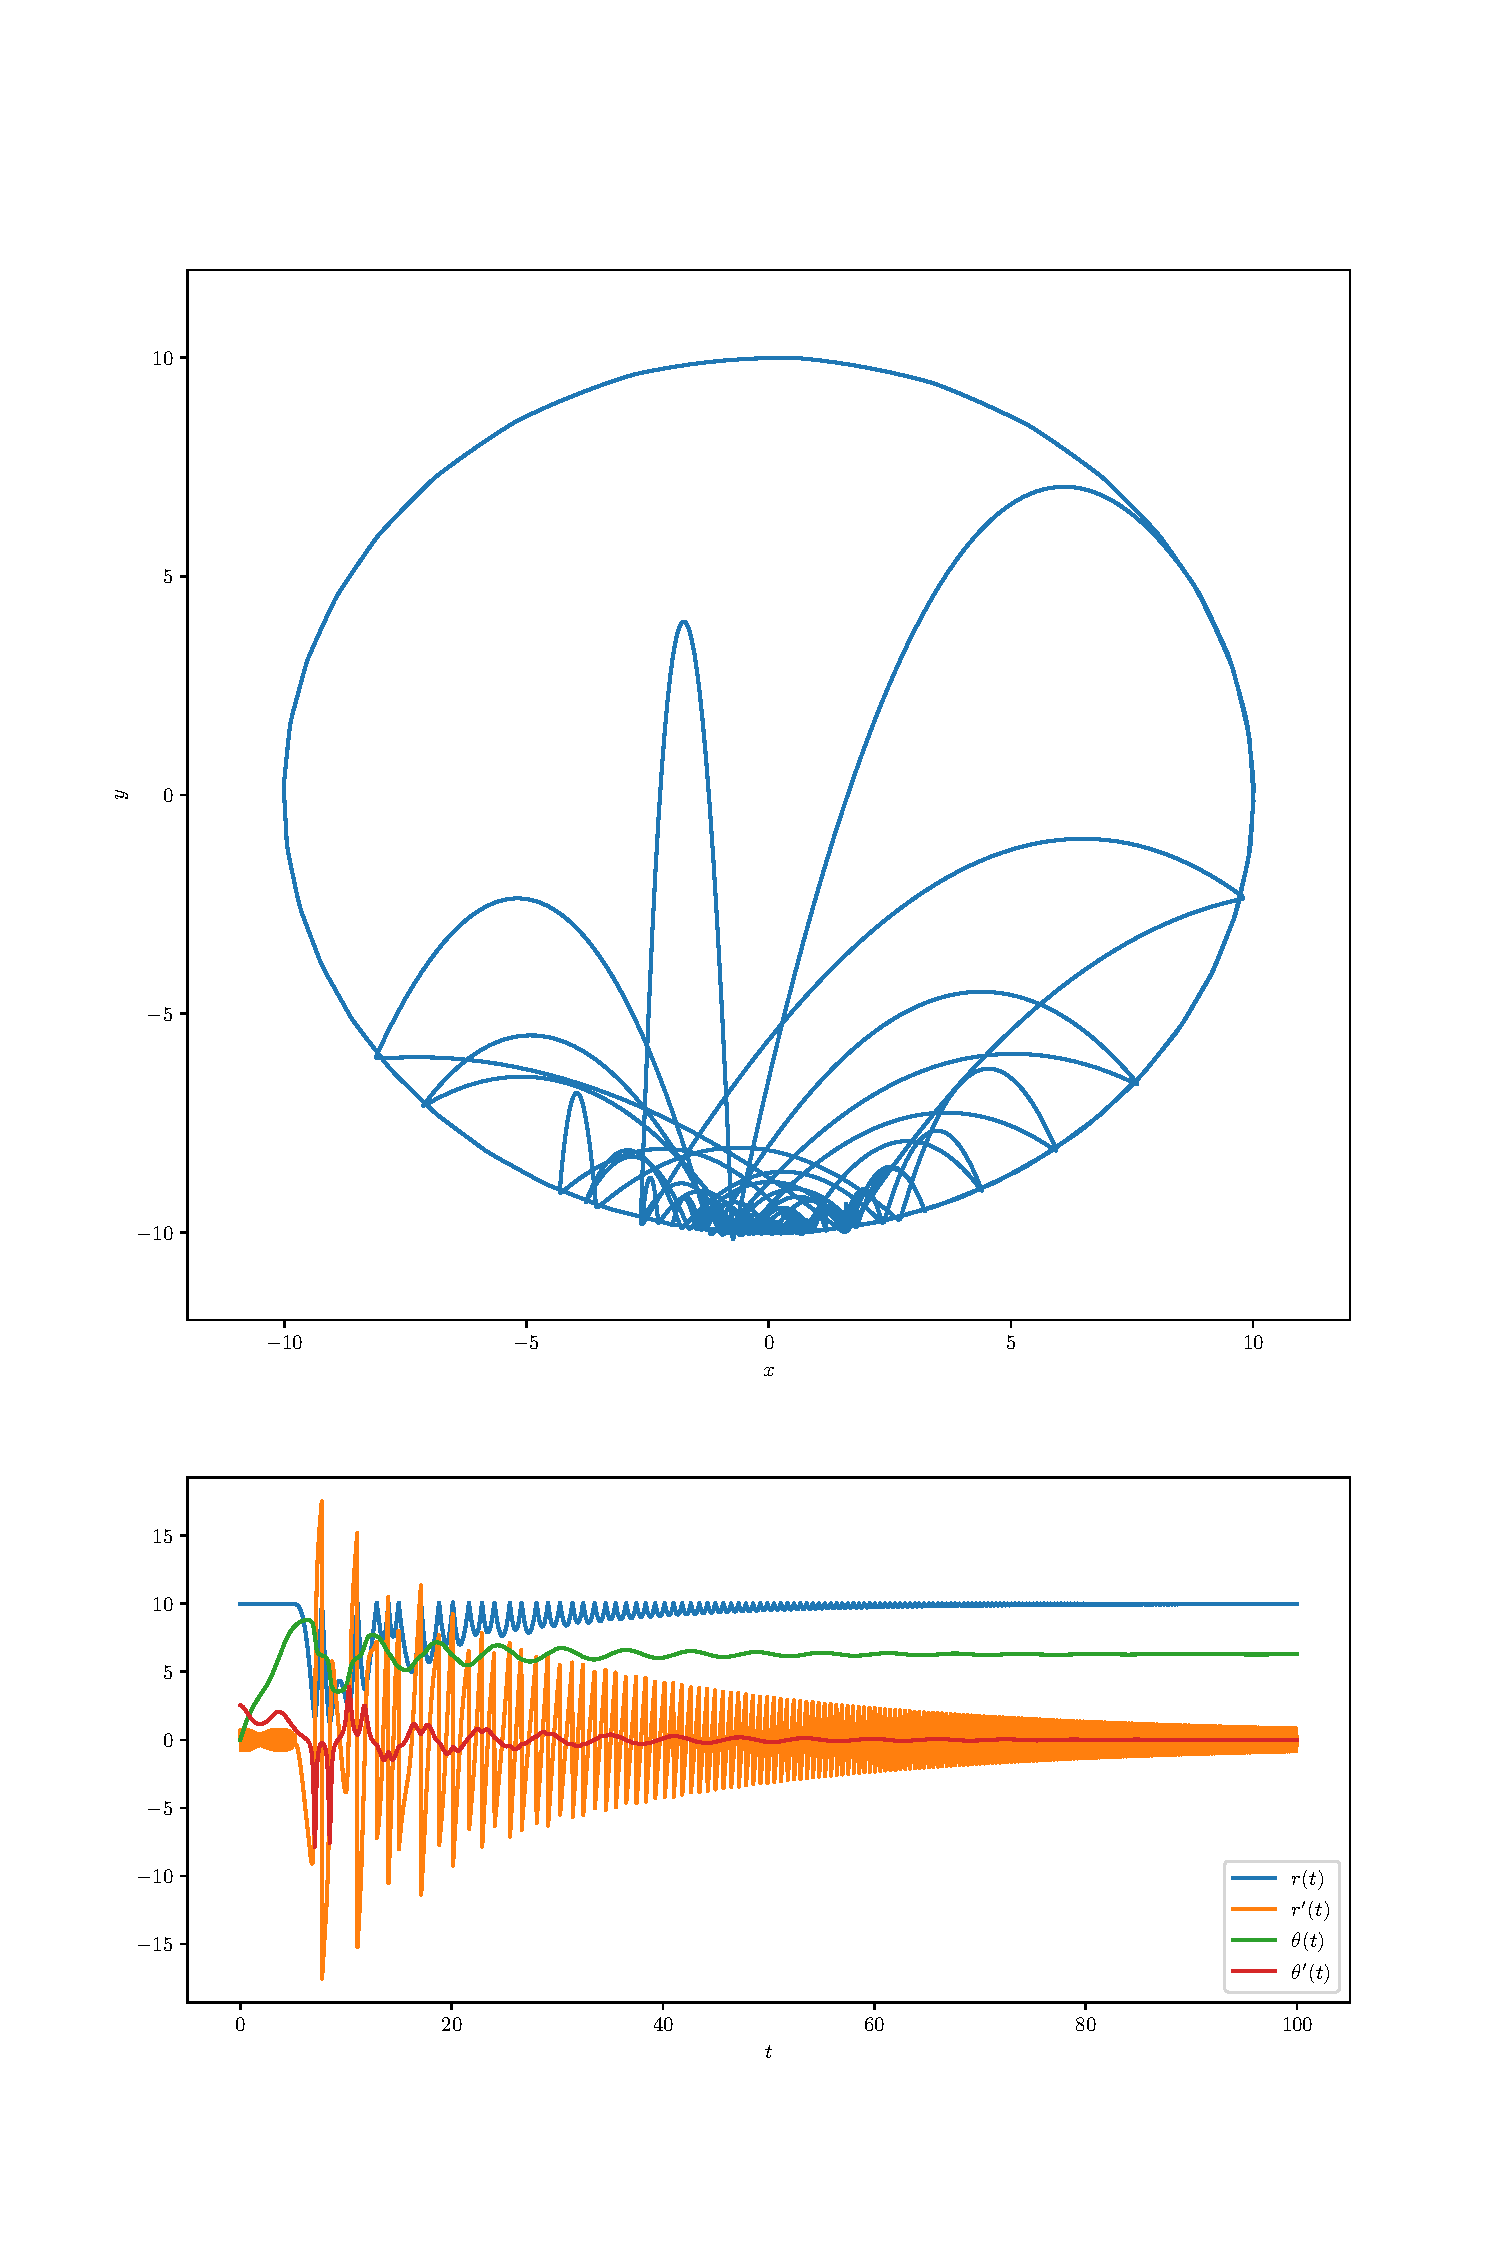
\includegraphics[width=0.8\textwidth]{fig.pdf}
  \end{center}
  \caption{\label{fig:f1} 4$^\mathrm{th}$-order Runge-Kutta approximation of the tetherball system.}
\end{figure}

If I haven't yet convinced you how cool numerical methods are, hopefully this will. Imagine a bouncy tetherball that is restricted to move in one plane. There is a flexible string of negligible mass with one end rigidly fixed to the origin and the other end connected to a weight. Gravity acts on the entire system, and whenever the tether is stretched to its maximum length, it bounces back with equal and opposite force. Because we can, suppose aerodynamic drag also acts on the weight. This system is governed by the following second-order system of ODE's, where $r(t)$ is the distance from the weight to the origin and $\theta(t)$ is the angle between the weight and the vertical.
\begin{align*}
  r''(t) & = r(t)\qty(\theta'(t))^2 + g\cos\theta(t) + \frac{f_s}{m} - \frac{d}{m}r'(t) \\
  \theta''(t) & = -\frac{1}{r}\qty(g\sin\theta + 2r\theta'(t) + \frac{rd}{m}\theta'(t)) \\
  f_s & = \begin{cases}
    0 & r(t) \leq l \\
    k(l - r(t)) & r(t) > l
  \end{cases}, \qq{where} \\
    g & = \SI{10}{\meter\per\second^2} \qq{is the acceleration due to gravity,} \\
    m & = \SI{1}{\kilo\gram} \qq{is the mass attached to the tether,} \\
    l & = \SI{10}{\meter} \qq{is the length of the tether,} \\
    d & = \SI{0.1}{\kilo\gram\per\second} \qq{is the strength of the aerodynamic drag, and} \\
    k & = \SI{1000}{\newton\per\meter} \qq{is the springiness of the tether.}
\end{align*}

Suppose the weight is hanging still, and someone gives it a strong counterclockwise push. Experience would lead us to expect the weight to
\begin{enumerate}
  \item Complete a few orbits with the cable taught while it has sufficient kenetic energy,
  \item leave the circular orbit as its velocity decreases, with the cable going slack,
  \item fall freely until the string becomes tight again,
  \item bounce erratically a few times as the cable's elasticity deflects the weight's velocity, and
  \item return to a steady hang.
\end{enumerate}

Any symbolic/closed-form solution that describes the weight's position as a function of time would be horrendous. (Even a pendulum simply swinging has no closed-form solution.) Therefore, we should use a numerical solver to model this situation. Applying the 4$^\mathrm{th}$-order Runge-Kutta Method to this system over $t \in [0, 100]$seconds with a step size $h = 0.0001$ and the initial conditions 
\[r(0) = \SI{10}{\meter} \quad r'(0) = \SI{0}{\meter\per\second} \quad \theta(0) = \SI{0}{\radian}, \qq{and} \theta'(0) = \SI{2.55}{\radian\per\second}\]
produces the results in figure \ref{fig:f1}. The result indeed is how we would expect a tetherball to behave.

\nocite{burdenc2011}
\nocite{greenbaum2012}
\nocite{press2007}
\nocite{suli2010}

\bibliography{refs.bib}

\end{document}
